


\section{Adversarial learning}
\label{sec:adversarial_learning}

	This section is the main contribution of the thesis. We'll see how how an idea of adversarial learning can be applied on a shallow-neural-network. This Idea was first developed by Ian J. Goodfellow, Jonathon Shlens and Christian Szegedy. They proposed an adversarial training on a shallow-feed-forward-neural-network. Along the paper\cite{goodfellow2014explaining}, they emphasize the be benefits of this method applied to a training on the MNIST dataset\cite{lecun-mnist}. Thanks to their adversarial learning, they obtained a better accuracy on the test set.


	
	\subsection{Intuition}
	\label{sub:intuition}
		With adversarial learning, we train our classifier to resit to samples that could confuse it. On the paper mentioned above\cite{goodfellow2014explaining}, the authors noticed that some adversarial modifications could be made up to fool drastically the classifier. If you were allowed to twist the pixels' values by $.7\%$, and chose carefully these values, you could mislead your classifier from a $95\%$ accuracy to a low $.7\%$. The twist they proposed was adversarial in the sense that they elected a twist given the current classifier. In other words, it's by knowing the intra-sec properties and weights of the model that they created the adversarial twists. These twists are computed with some math and will be detailed on section \ref{sec:creating_the_adversarial_samples}.

		To take advantage of this observation, we will train our model, not on the casual dataset, but on an adversarial version of it. To be more concrete: instead of forward-propagating the input sample through the model and get the prediction out of it, we will twist the input sample and forward-propagate it. The cost will get is the one of the adversarial samples and not of the original dataset.

		With this modification we hope that the classifier will learn, on the one hand, to recognize a class, like it would normally do, but on the other hand, will learn the differences between classes so that it can better discriminate them. 

		

	\subsection{Creating the adversarial samples}
	\label{sec:creating_the_adversarial_samples}
		The adversarial samples will be created from the original samples. We'll allow ourself to modify the pixels by some values. For instance, for an image, if pixels are coded with values between $0$ and $255$ ($0$ being black and $255$ white) we will allow ourselves to modify the pixels values by $\epsilon_{\text{adv}} \times 255$ so that the image looks the same. The modifications will be based on our feed-forward models weights biases and cost function. Concretely, the adversarial modifications will be equal to:
		$$ \eta = \epsilon_{\text{adv}} \times \text{sign}(\nabla_x \text{Cost}(\boldsymbol{W},\boldsymbol{x},\boldsymbol{y})) $$
		So that the adversarial samples $\boldsymbol{x}$ becomes:
		$$ \tilde{\boldsymbol{x}} = \boldsymbol{x} + \eta $$
		To create an adversarial sample we compute the derivative of the model 


	\subsection{Adversarial sample on our simple example}
	\label{sub:adversarial_sample_on_the_simple_example}
		Lets now build an example of adversarial sample. As always, we'll use the simple example we've build up (visible on section \ref{sec:weight_initialisation_on_simple_example}) and the sample $x^1$. From those two elements, we'll build-up the adversarial sample corresponding to it.

		We aim at deriving the cost of the model with respect to the inputs $x$. Luckily, we are able to re-use the back-propagation algorithm to compute the derivation. With the notation of section \ref{sec:back_propagation}, we have:
		\begin{equation}
			\begin{split}
				\frac{\nabla_{\boldsymbol{x}} C}{\partial \boldsymbol{x} } 
				&= \frac{\partial \boldsymbol{z}^1}{\partial \boldsymbol{x}} \frac{\partial C}{\partial \boldsymbol{z}^1 } \\
				&= \frac{\partial \left({\boldsymbol{w}^1}^T \boldsymbol{x} + \boldsymbol{b}^1 \right)}{\partial \boldsymbol{x}} \cdot \boldsymbol{\delta}^1 \\
				&= \boldsymbol{W}^1 \cdot \boldsymbol{\delta}^1
			\end{split}
		\end{equation}

		And the modified sample which is the sum of the sample plus a twist $\eta$ is:
		\begin{equation}
			\begin{split}
				\tilde{\boldsymbol{x}}
				&= \boldsymbol{x} + \eta \\
				&= \boldsymbol{x} + \epsilon_{\text{adv}} \times \text{sign}(\nabla_{\boldsymbol{x}} C) \\
				&= \boldsymbol{x} + \epsilon_{\text{adv}} \times \text{sign}( \boldsymbol{W}^1 \cdot \boldsymbol{\delta}^1 )
			\end{split}
			\label{eq:sample_twist}
		\end{equation}

		At this point, we know how to compute the compute an adversarial sample. From the last equation, it doesn't clearly appears that an adversarial sample depends on the variables of the model. Taking a closer look into it, we have that an adversarial sample depends on all the variables present on the model. The neurons' weights appears twice. First on the the back-propagation and then on the forward-propagation (the cost) and the biases appears once on the forward-propagation. We also have that the sample class is present on the cost. Therefore, the adversarial sample needs an entire knowledge on the model and on the samples.

		Lets apply this to sample $\boldsymbol{x}^1$ with $\epsilon_{\text{adv}} = .07$:
		\begin{equation}
			\begin{split}
				\widetilde{\boldsymbol{x}^1}
				&= \boldsymbol{x}^1 + \epsilon_{\text{adv}} \times \text{sign}( \boldsymbol{W}^1 \cdot \boldsymbol{\delta}^1 ) \\
				&= \boldsymbol{x}^1 + .07 \times \text{sign}
				\left( \left( \begin{matrix}
				-10 	& -10 	& 10 \\
				-10 	& 10 	& -10 \\
				20 		& 10 	& 10 \\
				\end{matrix} \right) \cdot
				\left( \begin{matrix}0 \\ 0.003 \\0.003  \end{matrix} \right) \right)\\
				&= \left( \begin{matrix} 0 \\   0 \\ 1  \end{matrix} \right) +
				\left( \begin{matrix}0.07 \\0.07 \\0.07 \end{matrix} \right) \\
				&= \left( \begin{matrix}0.07 \\0.07 \\1.07 \\\end{matrix} \right)
			\end{split}
		\end{equation}

		From this example we can see the adversarial twist put noise in a direction to confuse the model ?? why not decrease of $-.03$ augmented la loss for this given that.
		With this example, the benefits of adversarial learning are not clearly visible but we hope that the process underlining adversarial learning is understood.



	\subsection{MNIST}
	\label{sub:MNIST}
		
		The first dataset we're going to evaluate is the MNIST dataset\cite{lecun-mnist}. This dataset is composed by 70k images representing digits going from 0 to 9. Each of the images has $28*28$ black and white pixels. For each pixels is given a value in between 0 and 1 stating how bright is the pixel. The task, given this dataset, is to classify the samples into the 10 classes they belong in. For our needs, we discomposed the dataset into 3 sets: a training-set composed by 50k samples, a validation-set composed by 10k samples and a testing-set composed by 10k samples. 

		From our observations, this dataset is similar to a baseline in machine learning for testing algorithms in image processing. The reason is that it has been around for a long time and that it's big and small enough to quickly and accurately test new ideas related to this domain. It's for this reason that we'll make most of our tests using this dataset.

		Lets now get to adversarial learning. On their paper\cite{goodfellow2014explaining}, the authors used adversarial-learning in conjunction with other techniques. In order separate adversarial-learning from any anther technique, we've decided to re-implement the shallow-neural-network without any method that could be assimilated as a regularization. Concretely, the authors of the paper used two methods that function together called maxout and dropout. Dropout is considered to regularize the network. For this reason we removed it such that our net is only composed by the pixels inputs, the hidden ReLU layer and the softmax output layer. \Fref{fig:mnist_net} is a graphical representation of the MNIST net we used.

		\begin{figure}
			\centering
			\def\layersep{3cm}
			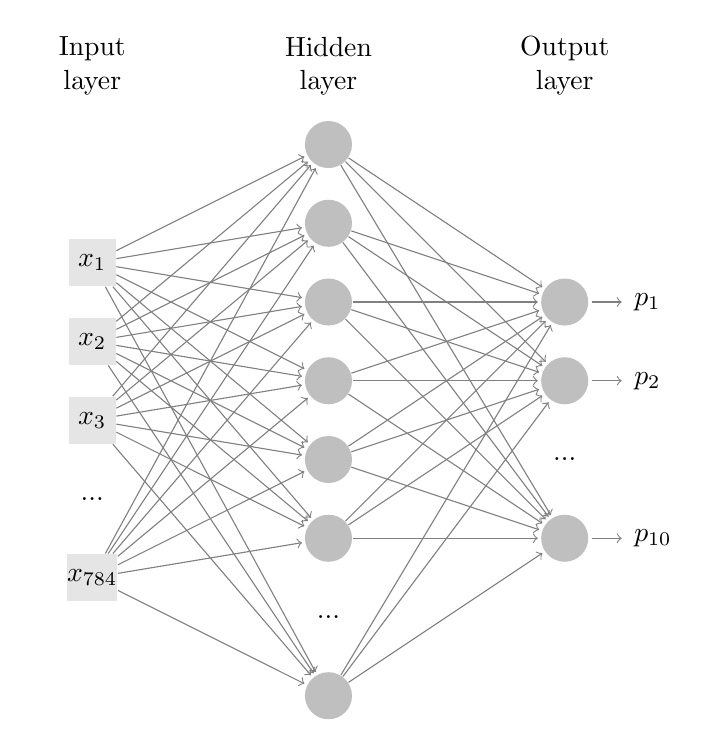
\begin{tikzpicture}[shorten >=1pt,->,draw=black!50, node distance=\layersep]
			    \tikzstyle{every pin edge}=[<-,shorten <=1pt]
			    \tikzstyle{neuron}=[circle,fill=black!25,minimum size=17pt,inner sep=0pt]
			    \tikzstyle{annot} = [text width=4em, text centered]
			    \tikzstyle{pixel} = [rectangle, fill=black!10,minimum size=17pt,inner sep=0pt]


			    %%%%%%%%%%%%%%%%%%%%%%%%%%%%%%%%%%%%%%%%%%%% 
			    %%% DRAW THE NODES
			    %%%%%%%%%%%%%%%%%%%%%%%%%%%%%%%%%%%%%%%%%%%%
			    \foreach \name / \y in {1,...,3}
			        \node[pixel] (I-\name) at (0,-1.5-\y) {$x_{\y}$};
		        \node[]      (I-4) at (0,-1.5-4) {...};
	            \node[pixel] (I-5) at (0,-1.5-5) {$x_{784}$};


			    \foreach \name / \y in {1,...,6}
			    	\node [neuron] (H1-\name) at (\layersep,-\y cm) {};
		    	\node []       (H1-7) at (\layersep,-7 cm) {...};
		    	\node [neuron] (H1-8) at (\layersep,-8 cm) {};

		       	
			    \node[neuron,pin={[pin edge={->}]right:$p_{1}$}, right of=H1-3] (O-1) {};
			    \node[neuron,pin={[pin edge={->}]right:$p_{2}$}, right of=H1-4] (O-2) {};
			    \node[right of=H1-5] (O-3) {...};
			    \node[neuron,pin={[pin edge={->}]right:$p_{10}$}, right of=H1-6] (O-4) {};

			    %%%%%%%%%%%%%%%%%%%%%%%%%%%%%%%%%%%%%%%%%%%% 
			    %%% DRAW THE PATHS
			    %%%%%%%%%%%%%%%%%%%%%%%%%%%%%%%%%%%%%%%%%%%%
			    \foreach \source in {1,...,3,5}
			        \foreach \dest in {1,...,6,8}
			            \path (I-\source) edge (H1-\dest);

			    \foreach \source in {1,...,6,8}
			    	\foreach \dest in {1,...,2,4}
				        \path (H1-\source) edge (O-\dest);

			    % Annotate the layers
			    \node[annot,above of=H1-1, node distance=1cm] (hl1) {Hidden layer};
			    \node[annot,left of=hl1] {Input layer};
			    \node[annot,right of=hl1] {Output layer};
			\end{tikzpicture}
			\caption{Graphical model of a MNIST net}
			\label{fig:mnist_net}
		\end{figure}

		\subsubsection{Playing with neuron quantities}
		\label{ssub:playing_with_neuron_quantities}
			One of the first experiment we got interested in knowing which parameters should be used to train the neural network. We would expect that the size of the hidden layer has a direct impact on the predictions and on the accuracy of the model. We would therefore try different layer sizes and see which ones were over and under fitting. We also want to know if one of the adversarial or usual training would under or over-fit before the other given the same amount of neurons. If one were to under-fit longer than the other, it would imply it need to learn more functions than the other model to be accurate.

			In other words, if both of the models stops under-fitting on the same time, it would probably mean that both of the models learn the same amounts of functions, but one would be more accurate than the other. On the other hand, if a model (A) under-fits longer than the other model (B) it would probably mean that it (A) needs to learn more functions to accurate than the other model (B).

			For this reason, the we've trained MNIST on models with different amount of weights. Each of the adversarial examples are trained with $\epsilon_{\text{adv}} = .25$. The graph on \fref{fig:mnist_neurons} shows the evolution of the accuracy and the confidence for the adversarial and non-adversarial models while increasing the amount of neurons. As one could expect, the accuracy is defined as :
			$$\text{acc} = \frac{\text{\#correct guesses}}{\text{\#samples}}$$ 
			And the confidence reflects how much the model was sure of which ever predictions it made 
			$$\text{conf} =  \text{mean}( \text{argmax} (\text{predictions}))$$

			TODO: ANALYSIS
			\begin{figure}
				\centering
				\includegraphics[width=0.7\textwidth]{/home/marc/git/MI10_adversarial_training/training_test/MLP3/mem/bar_acc_all.png}
				\caption{Comparing the amount of neurons' impact on non-adversarial and adversarial models. Every pair represent a non-adversarial-learning and an adversarial-learning trained with a certain amount of hidden neurons.}
				\label{fig:mnist_neurons}
			\end{figure}



		\subsubsection{Playing with adversarial epsilon}
		\label{ssub:playing_with_adversarial_epsilon}
			The Adversarial learning we use relies on an epsilon, the one we've noted $\epsilon_{\text{adv}}$:
			$$ \boldsymbol{x} + \epsilon_{\text{adv}} \times \text{sign}(\nabla_{\boldsymbol{x}} C) $$
			In this subsection, we want to evaluate the impact of this value on the learning. We are going to expose the learning of a 800 hidden-neurons net trained with different $\epsilon_{\text{adv}}$. Even though, we expect an increased accuracy with an increased epsilon, we don't have any idea on which epsilon would be better. 

			TODO: 800 + MANY EPSILONS_ADV

			\begin{figure}
				\centering
				\includegraphics[width=0.7\textwidth]{/home/marc/git/MI10_adversarial_training/training_test/MLP3/mem/plot_test_800.png}
				\caption{Evaluate non-adversarial and adversarial models of 800 hidden neurons .}
				\label{fig:mnist_neurons}
			\end{figure}


		\subsubsection{Compare to noisy dataset} 
		\label{ssub:compare_to_noisy_dataset}
			One of the objective mentioned for adversarial-learning was to diminish the linearity of the network: The authors of \cite{goodfellow2014explaining} said that usual networks were not able to understand the underlining nature of a class because it was too much dependent on the underlining distribution of the data present on the dataset. This dependency was described with too much linearity on the network to learn the underlining dataset. It's because of this over-linearity that adversarial samples were so good at fooling the models.

			On this subsection, we want to see if, effectively, the model is better at generalizing. To do this, we are going to compare a non-adversarial model (A) with an adversarial model (B) on a modified test-set. We are going to modify the original test-set by twisting each pixels by a random value. With this technique we'll produce few test-sets and test every of them on model A and B. The random value mentioned right before comes from a normal distribution with a given standard deviation. It's these deviations that is going to change from $0$ to $.3$ to produce the different test-sets.
			
			\begin{figure}
				\centering
				\includegraphics[width=0.7\textwidth]{/home/marc/git/MI10_adversarial_training/training_test/MLP3/mem/plot_test_800.png}
				\caption{Evaluate non-adversarial and adversarial models of 800 hidden neurons on noisy test-sets with different standard deviations.}
				\label{fig:mnist_neurons}
			\end{figure}



		\subsubsection{Train with noisy dataset} % (fold)
		\label{ssub:train_with_noisy_dataset}
			Here we want to see how is adversarial-learning doing compared to another idea. Right before we mentioned the motivation for adversarial-learning (too much dependence on underlining distribution). Adversarial-learning came as an idea to be less dependent on this underlining distribution. On this section, we are going to introduce noise on the learning dataset 
			Here we try another learning technique to compare with adversarial-learning. As a recall, adversarial-learning modified the input samples towards a worst case prediction given the model. Now, instead of modifying the input sample by this worst case sample, we'll modify the sample by a random noise. The random noise added to the learning dataset will be under a normal distribution with a standard deviation of $.25$. We don't necessary expect this learning to be better at classifying but we hope that it can better resist to adversarial samples. If it does, it could support that usual training is too much linear.

			\begin{figure}
				\centering
				\includegraphics[width=0.7\textwidth]{/home/marc/git/MI10_adversarial_training/training_test/MLP3/mem/plot_test_norm_800.png}
				\caption{Evaluate casual, adversarial and noisy models of 800 hidden neurons on noisy test-sets and adversarial datasets.}
				\label{fig:mnist_neurons}
			\end{figure}

			
		\subsubsection{Visualizing weights} % (fold)
		\label{ssub:visualizing_weights}
			We've also tried to compare the weights of each of the 
		

	

	on the cifar10 dataset

	on an other dataset
	% # => 150 -> yes
	% 0.511660728731
	% 0.510628044268

	% # => 120 -> no
	% 0.510774341233
	% 0.511152992203

	% # => 100 -> no
	% 0.51174678577
	% 0.511781208585

	% # => 100 -> yes
	% 0.510800158345
	% 0.510301027521

	% # => 80 -> yes
	% 0.510757129826
	% 0.510671072787

	% # => 60 -> no
	% 0.512469664894
	% 0.512521299117

	% # => 60 -> no
	% 0.510352661744
	% 0.511677940139
